\documentclass[11pt,a4paper]{article}

\usepackage{fontspec}
\setmainfont{Times New Roman}
\usepackage[margin=0.85in,headheight=14pt]{geometry}
\usepackage{microtype}
\usepackage{amsmath,amssymb}
\usepackage{graphicx}
\usepackage{xcolor}
\usepackage{booktabs}
\usepackage{tabularx}
\usepackage{array}
\usepackage{enumitem}
\usepackage{listings}
\usepackage{tikz}
\usetikzlibrary{arrows.meta,positioning,fit,calc,shapes.geometric}
\usepackage{pgfplots}
\pgfplotsset{compat=1.18}
\usepackage{fancyhdr}
\usepackage{hyperref}
\usepackage[nameinlink,noabbrev]{cleveref}

\definecolor{primaryblue}{RGB}{30,58,138}
\definecolor{midblue}{RGB}{59,130,246}
\definecolor{lightblue}{RGB}{239,246,255}
\definecolor{darkgray}{RGB}{51,65,85}
\definecolor{lightgray}{RGB}{248,250,252}
\definecolor{teal}{RGB}{13,148,136}
\definecolor{orange}{RGB}{234,88,12}
\definecolor{redtone}{RGB}{185,28,28}

\hypersetup{
    colorlinks=true,
    linkcolor=primaryblue,
    citecolor=primaryblue,
    urlcolor=midblue,
    pdftitle={SonicDrop: Acoustic Data Communication},
    pdfauthor={Reza Ahmadizadeh}
}

\pagestyle{fancy}
\fancyhf{}
\lhead{\small SonicDrop: Acoustic Data Communication}
\rhead{\small Technical Project Report}
\cfoot{\thepage}
\setlength{\parskip}{0.45em}
\setlength{\parindent}{0pt}
\setlist[itemize]{leftmargin=1.5em,itemsep=0.2em,topsep=0.25em}
\setlist[enumerate]{leftmargin=1.8em,itemsep=0.25em,topsep=0.25em}

\tikzset{
    block/.style={draw=primaryblue,fill=lightblue,rounded corners=2pt,
        align=center,minimum height=0.9cm,text width=2.35cm,font=\small},
    titlebox/.style={draw=primaryblue,fill=lightblue,rounded corners=3pt,
        align=center,minimum width=3.7cm,minimum height=1.35cm,
        text width=3.25cm,font=\small},
    architecturebox/.style={draw=primaryblue,fill=lightblue,rounded corners=3pt,
        align=center,minimum width=2.65cm,minimum height=1.1cm,
        text width=2.35cm,font=\footnotesize},
    smallblock/.style={draw=darkgray,fill=lightgray,rounded corners=2pt,
        align=center,minimum height=0.75cm,text width=1.65cm,font=\footnotesize},
    arrow/.style={-{Stealth[length=2mm]},thick,draw=darkgray},
    dashedarrow/.style={-{Stealth[length=2mm]},thick,dashed,draw=orange},
    node distance=0.55cm and 0.45cm
}

\begin{document}

\begin{titlepage}
\centering
\vspace*{1.6cm}
{\Large\bfseries Technical Project Report\par}
\vspace{0.8cm}
{\Huge\bfseries\color{primaryblue} SonicDrop\par}
\vspace{0.35cm}
{\LARGE A Software-Defined Acoustic Data Transceiver\par}
\vspace{0.6cm}
{\large Reliable text and binary-image transfer over a sound channel\par}
\vspace{1.8cm}

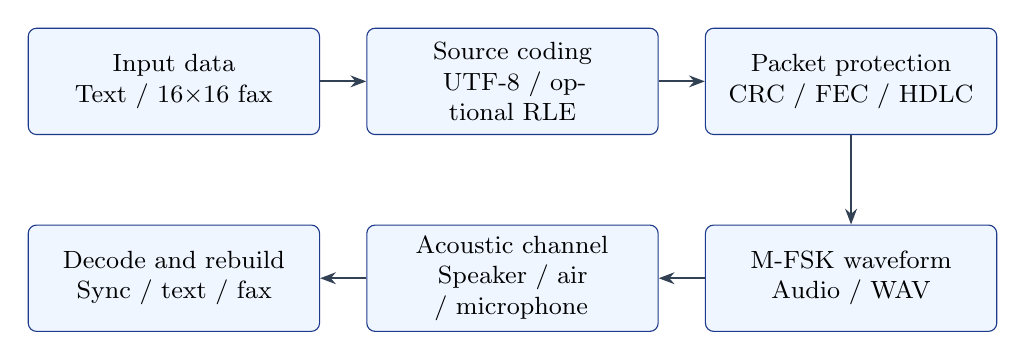
\begin{tikzpicture}[>=Stealth]
    \node[titlebox] (input) at (1.85,0) {Input data\\Text / 16$\times$16 fax};
    \node[titlebox] (source) at (6.15,0) {Source coding\\UTF-8 / optional RLE};
    \node[titlebox] (packet) at (10.45,0) {Packet protection\\CRC / FEC / HDLC};
    \node[titlebox] (modem) at (10.45,-2.5) {M-FSK waveform\\Audio / WAV};
    \node[titlebox] (channel) at (6.15,-2.5) {Acoustic channel\\Speaker / air / microphone};
    \node[titlebox] (receiver) at (1.85,-2.5) {Decode and rebuild\\Sync / text / fax};
    \draw[arrow] (input)--(source);
    \draw[arrow] (source)--(packet);
    \draw[arrow] (packet)--(modem);
    \draw[arrow] (modem)--(channel);
    \draw[arrow] (channel)--(receiver);
\end{tikzpicture}

\vfill
\begin{tabular}{rl}
    \textbf{Author:} & Reza Ahmadizadeh \\
    \textbf{Project:} & Acoustic Modem (SonicDrop) \\
    \textbf{Implementation:} & Python, Django, NumPy, browser audio APIs \\
    \textbf{Report date:} & \today
\end{tabular}
\vspace*{1.4cm}
\end{titlepage}

\begin{abstract}
SonicDrop is a software-defined modem and web application for sending short text messages and small binary images through sound. The sender converts application data into packets, adds a compact header and CRC-8, optionally applies Run-Length Encoding (RLE) and Hamming(7,4) forward error correction, frames the bit stream using HDLC-style flags and bit stuffing, and synthesizes a mono M-FSK waveform. The receiver accepts a WAV recording or microphone audio, detects candidate tones, searches several symbol-timing offsets, checks frames, repairs correctable bit errors, and reconstructs packet content. The interface also exposes simulated channel noise, signal metrics, frame inspection, and a browser-coordinated acoustic ACK/NACK demonstration. This report describes the implemented pipeline and its assumptions, distinguishes nominal calculations from measured results, and identifies important prototype limitations---in particular, the custom passkey transform is not production-grade cryptography and the browser ARQ demonstration is not a complete transport protocol.
\end{abstract}

\tableofcontents
\clearpage

\section{Introduction}
\label{sec:introduction}

Most consumer devices exchange data over radio networks or physical connectors. SonicDrop explores a different channel: a speaker emits a sequence of audio tones and a microphone records them. The design is intended as an educational prototype for short-range, ad-hoc communication, signal-processing experiments, and visualization of link-layer techniques. It does not require the two endpoints to share Wi-Fi or Bluetooth, although the current web application uses a browser and a Django server to prepare and inspect transmissions.

An acoustic room is a difficult communication medium. Reflections can make delayed copies of a tone overlap later symbols; microphone and speaker responses are not flat across frequency; distance and orientation change received level; and unrelated sounds can mask the signal. SonicDrop addresses these issues with multiple tone choices, tapered symbol edges, a trimmed integration region at the receiver, per-carrier energy normalization, frame synchronization, error detection, optional FEC, and repeated packet boundaries.

\subsection{Project goals}
The implemented project demonstrates the following:
\begin{itemize}
    \item Encode UTF-8 text and a 16$\times$16 binary image as bits.
    \item Send bits using audible or near-ultrasonic 2-FSK and 4-FSK.
    \item Preserve frame boundaries and detect damaged frames using flags, bit stuffing, and CRC-8.
    \item Correct a single error in an individual Hamming(7,4) codeword when that option is enabled.
    \item Optionally compress bit strings with a simple, lossless RLE format.
    \item Generate WAV audio, record microphone audio in the browser, and decode uploaded WAV files.
    \item Display waveform, frame, BER, SNR, and theoretical channel-capacity information.
\end{itemize}

\subsection{Scope and terminology}
The words \emph{sender} and \emph{receiver} refer to the end-to-end roles. The Django application builds a transmission and returns an audio file; the browser can play it or record input. A user can also transfer the WAV file to another device and upload it for decoding. Some interface behavior---notably live packet display and ACK/NACK orchestration---is coordinated between browser contexts, so it should be understood as a demonstration layered around the audio pipeline, not as evidence of a fully autonomous network protocol.

\section{System overview}
\label{sec:architecture}

\Cref{fig:architecture} shows the logical path through the project. Encoding proceeds from left to right at the sender; decoding reverses the transformations at the receiver. The channel in between is the physical air path and may add noise, attenuation, timing offset, and multipath effects.

\begin{figure}[ht]
\centering
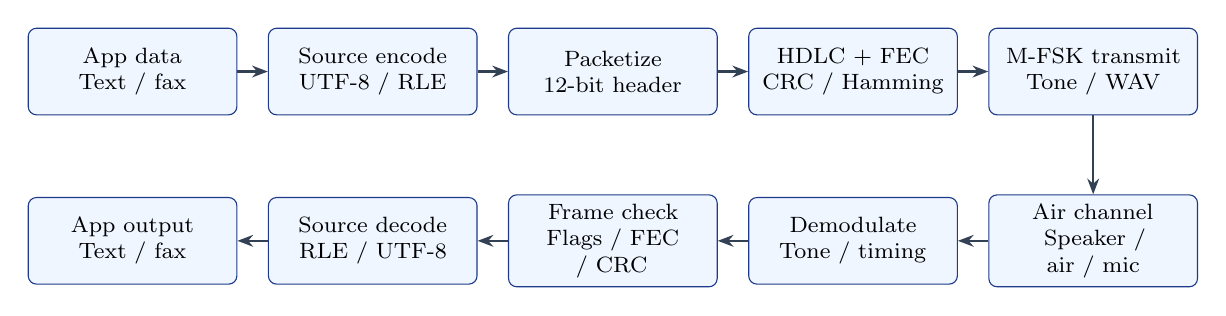
\begin{tikzpicture}[>=Stealth]
    \node[architecturebox] (app) at (1.325,0) {App data\\Text / fax};
    \node[architecturebox] (source) at (4.375,0) {Source encode\\UTF-8 / RLE};
    \node[architecturebox] (packet) at (7.425,0) {Packetize\\12-bit header};
    \node[architecturebox] (link) at (10.475,0) {HDLC + FEC\\CRC / Hamming};
    \node[architecturebox] (phy) at (13.525,0) {M-FSK transmit\\Tone / WAV};
    \node[architecturebox] (out) at (1.325,-2.15) {App output\\Text / fax};
    \node[architecturebox] (sourceout) at (4.375,-2.15) {Source decode\\RLE / UTF-8};
    \node[architecturebox] (linkout) at (7.425,-2.15) {Frame check\\Flags / FEC / CRC};
    \node[architecturebox] (phyout) at (10.475,-2.15) {Demodulate\\Tone / timing};
    \node[architecturebox] (air) at (13.525,-2.15) {Air channel\\Speaker / air / mic};
    \draw[arrow] (app)--(source);
    \draw[arrow] (source)--(packet);
    \draw[arrow] (packet)--(link);
    \draw[arrow] (link)--(phy);
    \draw[arrow] (phy)--(air);
    \draw[arrow] (air)--(phyout);
    \draw[arrow] (phyout)--(linkout);
    \draw[arrow] (linkout)--(sourceout);
    \draw[arrow] (sourceout)--(out);
\end{tikzpicture}
\caption{SonicDrop's implemented data path. Optional passkey processing is applied to packet content before link coding; reception filters and isolates audio before frame decoding.}
\label{fig:architecture}
\end{figure}

\subsection{Repository components}
\begin{table}[ht]
\centering
\small
\begin{tabularx}{\textwidth}{@{}lX@{}}
\toprule
\textbf{Component} & \textbf{Responsibility} \\
\midrule
\texttt{source\_coding.py} & UTF-8/bit conversion, image serialization, RLE, and the optional passkey-based bit transform. \\
\texttt{channel\_coding.py} & Packet headers, CRC-8, Hamming(7,4), HDLC flags and bit stuffing, shared-flag streams, and controlled error injection. \\
\texttt{modem\_phy.py} & M-FSK waveform generation, WAV serialization, tone-energy demodulation, stream search, and channel-rate calculations. \\
\texttt{views.py} & Django dashboard, transmit/analyze endpoint, WAV decode endpoint, and transmission logging. \\
\texttt{index.html} & Responsive sender, microphone receiver, fax canvas, signal lab, waveform plot, and browser-side coordination. \\
\texttt{models.py} & SQLite-backed transmission history and reported link metrics. \\
\bottomrule
\end{tabularx}
\caption{Primary implementation modules.}
\label{tab:modules}
\end{table}

\section{End-to-end operation}
\label{sec:operation}

\Cref{fig:sequence} summarizes a common send/receive session. The sender asks the Django endpoint for an encoded waveform. The result contains WAV bytes and diagnostic metadata; the browser plays it. Independently, a receiver can record audio or decode a WAV file. The decoder tests candidate modem settings, extracts packets, and reconstructs the most recent message identifier.

\begin{figure}[ht]
\centering
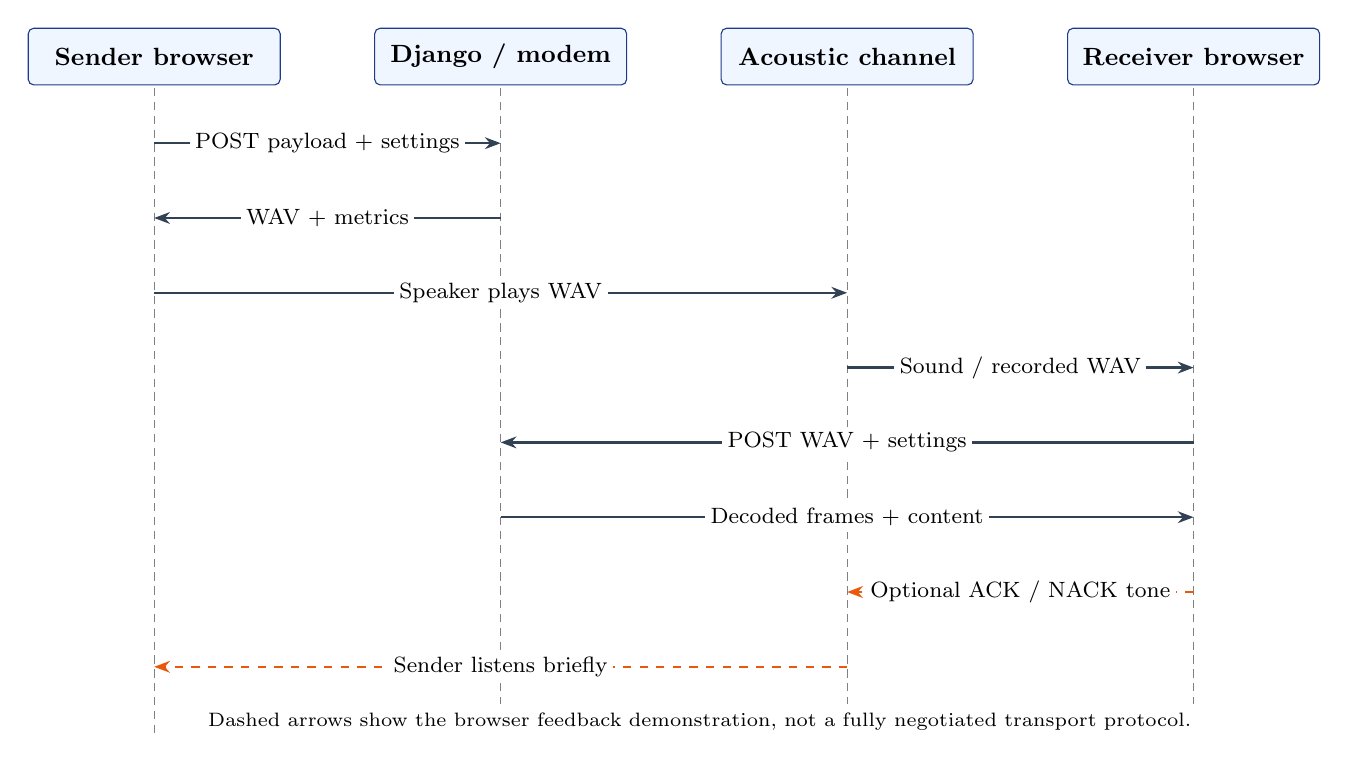
\begin{tikzpicture}[>=Stealth]
    \node[draw=primaryblue,fill=lightblue,rounded corners=2pt,minimum width=3.2cm,
        minimum height=0.72cm,align=center,font=\small\bfseries] at (0,0) {Sender browser};
    \node[draw=primaryblue,fill=lightblue,rounded corners=2pt,minimum width=3.2cm,
        minimum height=0.72cm,align=center,font=\small\bfseries] at (4.4,0) {Django / modem};
    \node[draw=primaryblue,fill=lightblue,rounded corners=2pt,minimum width=3.2cm,
        minimum height=0.72cm,align=center,font=\small\bfseries] at (8.8,0) {Acoustic channel};
    \node[draw=primaryblue,fill=lightblue,rounded corners=2pt,minimum width=3.2cm,
        minimum height=0.72cm,align=center,font=\small\bfseries] at (13.2,0) {Receiver browser};
    \draw[densely dashed,gray] (0,-0.4)--(0,-8.6);
    \draw[densely dashed,gray] (4.4,-0.4)--(4.4,-8.6);
    \draw[densely dashed,gray] (8.8,-0.4)--(8.8,-8.6);
    \draw[densely dashed,gray] (13.2,-0.4)--(13.2,-8.6);
    \draw[arrow] (0,-1.1)--node[fill=white,inner sep=2pt,font=\footnotesize]{POST payload + settings}(4.4,-1.1);
    \draw[arrow] (4.4,-2.05)--node[fill=white,inner sep=2pt,font=\footnotesize]{WAV + metrics}(0,-2.05);
    \draw[arrow] (0,-3.0)--node[fill=white,inner sep=2pt,font=\footnotesize]{Speaker plays WAV}(8.8,-3.0);
    \draw[arrow] (8.8,-3.95)--node[fill=white,inner sep=2pt,font=\footnotesize]{Sound / recorded WAV}(13.2,-3.95);
    \draw[arrow] (13.2,-4.9)--node[fill=white,inner sep=2pt,font=\footnotesize]{POST WAV + settings}(4.4,-4.9);
    \draw[arrow] (4.4,-5.85)--node[fill=white,inner sep=2pt,font=\footnotesize]{Decoded frames + content}(13.2,-5.85);
    \draw[dashedarrow] (13.2,-6.8)--node[fill=white,inner sep=2pt,font=\footnotesize]{Optional ACK / NACK tone}(8.8,-6.8);
    \draw[dashedarrow] (8.8,-7.75)--node[fill=white,inner sep=2pt,font=\footnotesize]{Sender listens briefly}(0,-7.75);
    \node[fill=white,font=\scriptsize,align=center,text width=12.8cm] at (6.9,-8.45)
        {Dashed arrows show the browser feedback demonstration, not a fully negotiated transport protocol.};
\end{tikzpicture}
\caption{Request, audio, decode, and optional feedback sequence.}
\label{fig:sequence}
\end{figure}

\subsection{Transmission endpoint}
The \texttt{/api/transmit/} endpoint accepts JSON containing the payload type, text or fax bits, carrier band, modulation order, symbol rate, delivery mode, and options for RLE, Hamming coding, noise, error injection, and passkey use. It constructs one or more packet payloads, frames them, synthesizes the complete audio stream, and returns a base64-encoded WAV plus packet timing and diagnostics. Transmission analysis for the signal lab is also performed in the server process.

\subsection{Reception endpoint}
The \texttt{/api/decode-wav/} endpoint accepts a WAV file and receiver settings. It reads mono PCM sample values from the WAV stream, tries a bounded list of modulation configurations, and returns the first configuration that yields valid frames. Frames are CRC-checked, their headers are parsed, optional passkey processing and RLE decoding are applied, and text or fax data are assembled by sequence number. If no valid frames are found, the endpoint returns an error rather than recovered application data.

\subsection{Live microphone and browser coordination}
The interface uses browser audio APIs to record microphone input and sends WAV recordings to the decode endpoint. A browser-side channel synchronizes settings and demo events across tabs. The sender can also open a short microphone window after playback to look for an ACK/NACK tone. Because live UI packet scheduling and some demonstration controls are coordinated by browser messages, a successful animation or displayed packet should not be confused with a successful independent acoustic decode; the decoded-WAV endpoint is the path that exercises recorded waveform recovery.

\section{Source coding and packet format}
\label{sec:source}

\subsection{Text and image representation}
Text is encoded as UTF-8, then represented as eight bits per byte. The decoder truncates incomplete trailing bytes and uses replacement characters for malformed UTF-8; a printable-text check filters likely-noisy results. The 16$\times$16 fax is flattened row by row to 256 binary pixel values. A zero/one pixel is serialized as one bit; the receiver reshapes the recovered sequence into the grid.

\subsection{Run-Length Encoding}
The RLE format represents each run as one bit for the repeated value followed by a seven-bit unsigned run length. A record is therefore eight bits long; runs are capped at 127 and longer runs are split. For example, a run of five ones is represented by the record \texttt{1 0000101}. RLE is optional for text, while fax data is RLE-encoded by the transmit implementation. It is effective for long runs (common in simple binary pictures), but can expand data that alternates frequently because every run consumes eight encoded bits.

\subsection{Packet header}
Each payload begins with a 12-bit header, followed by application content (or transformed content). \Cref{tab:header} documents the exact fields.

\begin{table}[ht]
\centering
\begin{tabular}{@{}clcl@{}}
\toprule
\textbf{Bit range} & \textbf{Field} & \textbf{Width} & \textbf{Meaning} \\
\midrule
0--2 & Message ID & 3 & Identifies a message; nonzero values 1--7 are generated. \\
3 & Delivery mode & 1 & Stream/word-oriented mode flag. \\
4 & Last packet & 1 & Marks the final packet in the message. \\
5 & Payload type & 1 & Fax flag; zero denotes text. \\
6 & Encrypted flag & 1 & Indicates that a passkey transform was applied. \\
7--11 & Sequence number & 5 & Packet number, represented modulo 32. \\
\bottomrule
\end{tabular}
\caption{The packet header packed by the channel-coding module.}
\label{tab:header}
\end{table}

In word-oriented mode, text is split into words and sent as a sequence of packets; full-message mode groups up to four words in each packet. Fax content is split into fixed-size chunks of compressed bits (32 bits in stream mode and 64 bits in full mode). Packet headers allow the receiver to order data and detect the final packet. The five-bit sequence field limits unambiguous numbering to 32 packet positions; this matters for worst-case fax patterns that compress poorly.

\subsection{Optional passkey transform and security limits}
When a non-empty passkey is supplied, the implementation derives a repeatable bit stream by hashing strings containing a version label, passkey, packet sequence as salt, and counter with SHA-256. It XORs that stream with the payload preceded by an eight-bit SHA-256-derived verification tag. The receiver regenerates the stream, XORs the result, and compares the tag. A packet sequence number is used as the salt so different packets in a message generally have different transform inputs.

\textbf{Security warning:} this is a project demonstration, not a vetted encryption or authentication scheme. The custom construction has no password-hardening KDF, uses a very short (8-bit) verification tag, has no standard AEAD guarantees, and can reuse keystream inputs when the same key and packet sequence recur. It must not be used to protect sensitive information. A production system should use a reviewed authenticated-encryption construction with nonce management and a password-based key derivation function where appropriate.

\section{Data-link framing and error control}
\label{sec:link}

\subsection{CRC-8}
The link layer appends an eight-bit CRC remainder computed with generator polynomial
\[
    G(x)=x^8+x^2+x+1 \qquad (\text{bit pattern }100000111).
\]
The CRC is calculated over the packet header and content before FEC. At the receiver, a zero remainder indicates that the received protected data passes the CRC check. CRC detects many accidental corruptions; it is not an error-correction code and should not be treated as cryptographic authentication.

\subsection{Hamming(7,4) forward error correction}
When enabled, the 12-bit header plus content and CRC are padded to a multiple of four bits and encoded in four-data-bit blocks. Three parity bits are placed in positions 1, 2, and 4, producing seven transmitted bits per four input bits. The decoder calculates a three-bit syndrome; a nonzero syndrome identifies a bit position to flip. This corrects one bit per seven-bit codeword. It does not reliably correct multiple errors in the same codeword, and such errors can be miscorrected; the CRC supplies a second integrity check after decoding.

The code rate is $4/7\approx0.571$ before CRC, framing, and bit-stuffing overhead. The extra redundancy increases transmission time but can recover isolated channel bit errors without requesting another copy.

\subsection{HDLC-style frame boundaries}
The channel coder constructs a frame from a 24-bit alternating preamble, the flag \texttt{01111110}, a protected body, and a closing flag. Within the body, bit stuffing inserts a zero after every run of five ones. The decoder removes stuffed zeros before FEC and CRC processing. This reduces the chance that body data will imitate the flag sequence. For multiple packets, the shared stream includes repeated flags between bodies for additional separation, then a short trailing preamble fragment.

\begin{figure}[ht]
\centering
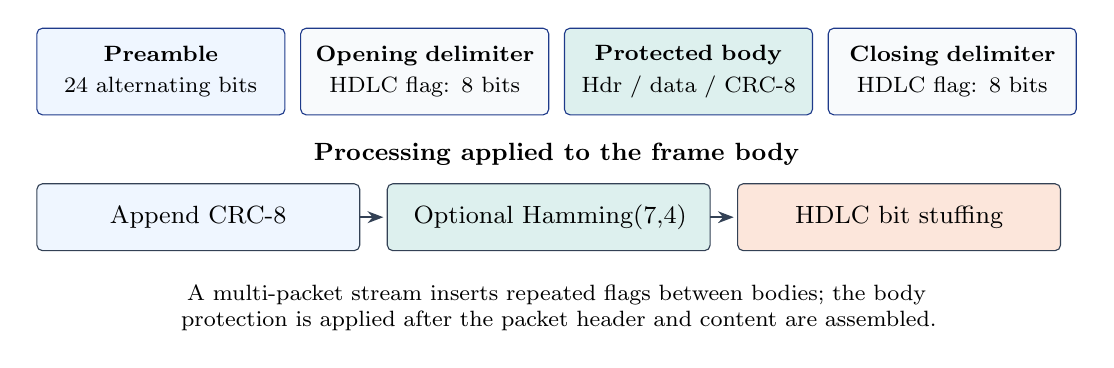
\begin{tikzpicture}[>=Stealth]
    \tikzset{framefield/.style={draw=primaryblue,rounded corners=2pt,
        minimum width=3.15cm,minimum height=1.1cm,text width=2.85cm,
        align=center,font=\footnotesize}}
    \node[framefield,fill=lightblue] at (1.575,0)
        {\textbf{Preamble}\\[2pt]24 alternating bits};
    \node[framefield,fill=lightgray] at (4.925,0)
        {\textbf{Opening delimiter}\\[2pt]HDLC flag: 8 bits};
    \node[framefield,fill=teal!14] at (8.275,0)
        {\textbf{Protected body}\\[2pt]Hdr / data / CRC-8};
    \node[framefield,fill=lightgray] at (11.625,0)
        {\textbf{Closing delimiter}\\[2pt]HDLC flag: 8 bits};
    \node[font=\small\bfseries] at (6.6,-1.05) {Processing applied to the frame body};
    \tikzset{protectionstep/.style={draw=darkgray,rounded corners=2pt,
        minimum width=4.1cm,minimum height=0.85cm,text width=3.8cm,
        align=center,font=\small}}
    \node[protectionstep,fill=lightblue] at (2.05,-1.85) {Append CRC-8};
    \node[protectionstep,fill=teal!14] at (6.5,-1.85) {Optional Hamming(7,4)};
    \node[protectionstep,fill=orange!15] at (10.95,-1.85) {HDLC bit stuffing};
    \draw[arrow] (4.1,-1.85)--(4.4,-1.85);
    \draw[arrow] (8.55,-1.85)--(8.85,-1.85);
    \node[font=\footnotesize,align=center,text width=13.2cm] at (6.6,-3.0)
        {A multi-packet stream inserts repeated flags between bodies; the body protection is applied after the packet header and content are assembled.};
\end{tikzpicture}
\caption{Equal-width frame fields and the order of body protection. Field widths are illustrative; only the stated preamble and flags have fixed bit lengths.}
\label{fig:frame}
\end{figure}

\subsection{Packet delivery and retransmission demonstration}
The interface labels its feedback feature as Hybrid ARQ. The browser can emit a 6.8\,kHz ACK tone or a 3.4\,kHz NACK tone and the sender can listen for those frequencies after playback. A forced-NACK option provides a demonstration path that corrupts a selected packet and retries a packet by sequence number; the sender permits at most one automatic retry in that UI flow. The decoder endpoint also returns ACK-related metadata when it has recovered valid frames.

This is not yet a complete selective-repeat ARQ protocol. It does not provide a robust on-air feedback packet with message/sequence identifiers, negotiated timeouts, retry limits across a session, duplicate suppression guarantees, or recovery of missing packets for every receive path. In particular, browser-local simulation, API analysis, and independent WAV reception have different levels of coupling. The report therefore describes ARQ as a prototype feedback demonstration, not as a guarantee of zero data loss.

\section{Physical layer}
\label{sec:phy}

\subsection{Modulation choices}
The physical layer uses $M$-ary frequency-shift keying. Each symbol selects one carrier; for $M=2$ a symbol carries one bit, and for $M=4$ a symbol carries two bits. The 4-FSK symbol mapping is \texttt{00}, \texttt{01}, \texttt{10}, \texttt{11} in the order of the four configured carrier frequencies. If a 4-FSK input contains an odd number of bits, the modulator pads one zero bit.

\begin{table}[ht]
\centering
\begin{tabularx}{\textwidth}{@{}llXrr@{}}
\toprule
\textbf{Mode} & \textbf{M} & \textbf{Carrier frequencies (Hz)} & \textbf{Bandwidth used} & \textbf{Bits/symbol}\\
\midrule
Audible & 2 & 2600, 3800 & 2000 Hz & 1\\
Audible & 4 & 2400, 3100, 3800, 4500 & 2600 Hz & 2\\
Near-ultrasonic & 2 & 14800, 15800 & 2000 Hz & 1\\
Near-ultrasonic & 4 & 14400, 15000, 15600, 16200 & 2400 Hz & 2\\
\bottomrule
\end{tabularx}
\caption{Carrier sets and bandwidth values configured in the physical layer.}
\label{tab:tones}
\end{table}

At sample rate $f_s$ and symbol rate $R_s$, the implementation uses
\[
    N_s=\left\lfloor\frac{f_s}{R_s}\right\rfloor
\]
samples per symbol. The default sample rate is 44.1\,kHz and the default symbol rate is 45 baud. The resulting nominal uncoded bit rate is
\[
    R_b=R_s\log_2(M).
\]
Thus, at 45 baud, 2-FSK carries 45 nominal bits/s and 4-FSK carries 90 nominal bits/s before framing, CRC, FEC, bit stuffing, and optional compression. These are configuration-derived rates, not measured application goodput.

\subsection{Waveform generation}
The modulator generates a sinusoid at the carrier selected by each symbol. It carries phase forward from symbol to symbol and applies a short raised-cosine taper at each symbol edge to reduce abrupt amplitude transitions. The resulting float waveform is scaled and converted to mono, signed 16-bit PCM WAV. For 4-FSK, an odd trailing bit is padded as noted above.

\begin{figure}[ht]
\centering
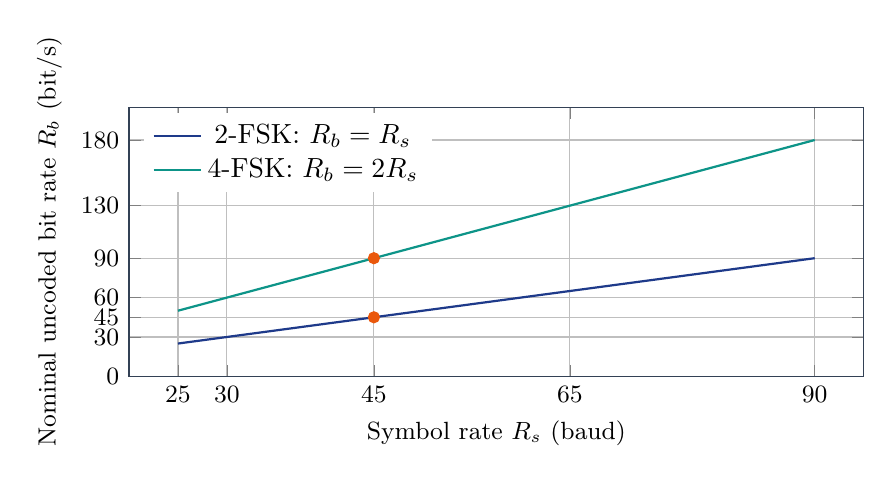
\begin{tikzpicture}
\begin{axis}[
    width=0.9\textwidth,
    height=5.0cm,
    xlabel={Symbol rate $R_s$ (baud)},
    ylabel={Nominal uncoded bit rate $R_b$ (bit/s)},
    xmin=20,xmax=95,ymin=0,ymax=205,
    xtick={25,30,45,65,90},
    ytick={0,30,45,60,90,130,180},
    grid=both,
    legend style={at={(0.02,0.98)},anchor=north west,draw=none,fill=white},
    axis line style={darkgray},
    tick label style={font=\small},
    label style={font=\small}
]
    \addplot[primaryblue,thick,domain=25:90,samples=2] {x};
    \addlegendentry{2-FSK: $R_b=R_s$}
    \addplot[teal,thick,domain=25:90,samples=2] {2*x};
    \addlegendentry{4-FSK: $R_b=2R_s$}
    \addplot[only marks,mark=*,mark size=2pt,orange] coordinates {(45,45) (45,90)};
\end{axis}
\end{tikzpicture}
\caption{Nominal modulation bit rate versus symbol rate, calculated from $R_b=R_s\log_2(M)$. Markers show the project's default 45-baud setting. The plot excludes protocol overhead and does not represent measured throughput.}
\label{fig:rate}
\end{figure}

\subsection{Demodulation and timing search}
For each symbol, the receiver discards an edge guard region (approximately 14\% of the symbol at each end) and correlates the remaining samples against in-phase and quadrature templates for each candidate carrier. The squared correlation magnitudes estimate tone energy. When enough symbols are present, each carrier's energy is normalized by a high percentile of its observed power to partially compensate for unequal speaker/microphone frequency response. The highest normalized-energy carrier is selected; low-energy symbols are squelched.

For WAV reception, the implementation removes the recording mean, applies an FFT band-pass mask around the configured carrier range, normalizes gain, and isolates an active burst using tone dominance. It then tries up to 20 offsets within one symbol interval. At each offset, the resulting bits are scanned for frame flags and checked with FEC and CRC. This search helps tolerate unknown start alignment, but is a bounded timing search rather than a full timing-recovery loop or channel equalizer.

\subsection{Audible versus near-ultrasonic operation}
The near-ultrasonic carrier set aims to reduce audible tones while remaining within the nominal Nyquist limit of a 44.1\,kHz sample rate. Real hardware may attenuate these frequencies strongly or reject them through built-in audio processing; some microphones, speakers, and codecs do not preserve them adequately. The audible setting is generally easier to observe and debug. Neither carrier mode should be assumed to work across all devices without measurement.

\section{Channel metrics and interpretation}
\label{sec:metrics}

The physical layer reports an estimated SNR in decibels, a nominal bit rate, a Nyquist rate, and a Shannon capacity estimate. In the code these estimates use the detected tone and residual competing-tone powers:
\[
    \mathrm{SNR}_{dB}=10\log_{10}\!\left(\frac{P_s}{P_n}\right),
\]
where $P_s$ is estimated average winning-carrier power and $P_n$ is average power in the other carrier hypotheses. The reported theoretical limits are
\[
    R_{\mathrm{Nyquist}}=2B\log_2(M), \qquad
    C_{\mathrm{Shannon}}=B\log_2(1+\mathrm{SNR}_{linear}),
\]
with configured bandwidth $B$. These are reference calculations under idealized assumptions; the acoustic channel is not guaranteed to satisfy those assumptions, and an estimated SNR is not a lab measurement of end-to-end bit error probability.

The transmit-and-analyze endpoint returns a clean synthesized WAV, then applies Gaussian noise and optional artificial bit flips to a separate first-frame copy for analysis. Its BER is computed by comparing that demodulated copy with the generated frame. This metric is useful for controlled tests but is not a field BER measurement. In the WAV receive path, the reported BER-like value is derived from corrected bits and a displayed frame length; it should not be interpreted as a complete statistical estimate over many independent packets.

\section{Web application and data persistence}
\label{sec:web}

Django exposes three routes: the dashboard at \texttt{/}, transmission analysis at \texttt{/api/transmit/}, and WAV decoding at \texttt{/api/decode-wav/}. NumPy implements waveform and spectral operations. The dashboard provides text and fax input, controls for carrier/modulation and link options, a recording receiver, WAV upload, a frame bit inspector, metrics cards, and a waveform plot. The fax grid is 16$\times$16 pixels.

Each transmit-and-analyze request creates a \texttt{TransmissionLog} record in SQLite with the chosen band, symbol-rate-related field, coding options, bit lengths, injected/corrected error counts, BER, SNR, theoretical rates, CRC result, and recovered/display label. The dashboard shows recent entries. This history supports experiments but is not a production telemetry or account system.

\section{Testing and evaluation}
\label{sec:testing}

The repository includes an engine demonstration that:
\begin{enumerate}
    \item Converts a UTF-8 test sentence into bits, frames it with CRC-8 and Hamming coding, injects artificial errors, and prints decoder correction and CRC results.
    \item Encodes and decodes an example binary image with RLE and verifies that the output bits match the input bits.
\end{enumerate}
The README documents Django's \texttt{manage.py check} and an optional speaker/microphone demo. These checks are not a cross-device benchmark; no range, error-rate, security, or hardware-compatibility guarantees are claimed.

\subsection{Reproducible local checks}
With project dependencies installed, the documented checks are:
\begin{lstlisting}[basicstyle=\ttfamily\small,frame=single,backgroundcolor=\color{lightgray}]
python manage.py check
python transceiver/engine/test_engine.py
\end{lstlisting}
For an end-to-end acoustic evaluation, record the emitted WAV with a second device at documented distance, orientation, volume, and environment settings. Repeat each condition over many packets, report both packet success rate and goodput, and retain the original recordings so decoding results can be reproduced.

\section{Limitations and future work}
\label{sec:limitations}

\subsection{Current limitations}
\begin{itemize}
    \item \textbf{Prototype cryptography:} the SHA-256/XOR transform and short tag are not safe for confidential data; use a standard authenticated-encryption library for any real security requirement.
    \item \textbf{Incomplete ARQ:} feedback and retry behavior are primarily a browser demonstration. It lacks a complete on-air protocol for identifiers, timeout policy, loss recovery, and duplicate handling.
    \item \textbf{Packet-size and sequence bounds:} the header has only five sequence bits. Highly alternating fax pixels can produce enough RLE records to exceed 32 packet positions.
    \item \textbf{Timing and channel model:} the receiver uses a finite phase search, energy detector, and simple spectral compensation. It does not estimate a full impulse response or continuously track clock drift.
    \item \textbf{Rate adaptation:} the code produces a recommended profile from SNR/BER thresholds; this recommendation is diagnostic and is not, by itself, a negotiated automatic change to an ongoing link.
    \item \textbf{Limited measurements:} synthetic error injection and the included engine demonstration do not establish acoustic range, robustness across rooms, or real-world throughput.
    \item \textbf{History field naming:} the transmit view currently stores effective bit rate in the database field named \texttt{baud\_rate}; historical values should not be read as symbol-rate measurements.
    \item \textbf{Input validation and deployment:} this is a local development application. Before public deployment, enforce request-size limits, validate all options, review CSRF/API policy, configure production secrets and allowed hosts, and use an appropriate server configuration.
\end{itemize}

\subsection{Recommended next steps}
\begin{enumerate}
    \item Add automated unit tests for CRC vectors, framing/unstuffing, single- and multi-bit Hamming cases, RLE edge cases, packet boundaries, encryption failure behavior, and modem round trips.
    \item Add a versioned frame format with payload length, robust message identifiers, and sequence numbers large enough for the supported maximum message size.
    \item Replace the custom passkey transform with a standard AEAD scheme and define a secure key derivation and nonce lifecycle.
    \item Specify an actual feedback frame or robust coded tone sequence, including packet identity, timeout, retry, and duplicate rules; test it on independent devices.
    \item Measure recorded audio across devices and environments. Publish sample rate, distance, volume, carrier set, baud rate, packet size, trials, error counts, and confidence intervals.
    \item Improve synchronization and channel estimation, and evaluate interleaving or stronger codes for burst noise and reverberation.
    \item Separate simulator-generated metrics from measurements on recordings in the UI and stored history.
\end{enumerate}

\section{Conclusion}
\label{sec:conclusion}

SonicDrop is an end-to-end educational acoustic modem: it turns application data into framed bit streams, maps those streams to audio tones, and provides a software receiver for recovering content from recordings. Its layered implementation makes source coding, packetization, CRC, optional FEC, M-FSK, signal metrics, and web presentation visible and testable. The included diagrams and rate plot describe the implemented algorithms and theoretical calculations rather than claiming a benchmark result. The project is a useful foundation for further experimentation, with cryptography, protocol completeness, acoustic evaluation, and stronger synchronization identified as the most important next steps.

\appendix
\section{Default configuration quick reference}
\label{app:defaults}
\begin{table}[ht]
\centering
\begin{tabularx}{\textwidth}{@{}lX@{}}
\toprule
\textbf{Parameter} & \textbf{Default / behavior} \\
\midrule
Sample rate & 44,100 samples/s; mono 16-bit PCM WAV output. \\
Symbol rate & 45 baud in the API defaults and initial interface control; the UI slider spans 25--90 baud in 5-baud steps. \\
Modulation & 4-FSK by default (two bits per symbol); 2-FSK is also selectable. \\
Carrier band & Audible by default; near-ultrasonic is selectable. \\
Hamming & Enabled by default; may be disabled. \\
Text RLE & Disabled by default; may be enabled. Fax content is always RLE encoded by the transmit pipeline. \\
Noise/error controls & The analysis endpoint supports configurable Gaussian noise and optional artificial single, multiple, or burst bit flips. \\
WAV receive search & Tries requested settings and several fallback configurations, then returns the first set of valid frames found. \\
\bottomrule
\end{tabularx}
\caption{Defaults and observable behavior in the current implementation.}
\end{table}

\end{document}
